% nastavenia prostredia
\documentclass[12pt,a4paper,titlepage,final]{report}
\usepackage[utf8]{inputenc}
\usepackage[T1, IL2]{fontenc}
\usepackage{graphicx}
\usepackage{epstopdf}
\usepackage{caption}
\usepackage[top=3cm, left=1cm, right=1cm, text={17cm, 24cm}, ignorefoot]{geometry}
\usepackage{color}
\usepackage{url}
\usepackage[bookmarksopen,colorlinks,plainpages=false,urlcolor=blue,unicode]{hyperref}

\begin{document}
	% define
	\def\authora{Michal Riša}
	\def\authorb{Pavel Macenauer}
	\def\emaila{xrisam01@stud.fit.vutbr.cz}
	\def\emailb{xmacen02@stud.fit.vutbr.cz}
	\def\docname{Firma2}
	\def\projname{Prvotná analýza a plán projektu}
	% titulna strana
	\begin{titlepage}
	\begin{center}
		\includegraphics[height=5cm]{img/logo.eps}
	\end{center}
	\vfill
	\begin{center}
		\begin{Large}
			\docname\\
		\end{Large}
		\bigskip
		\begin{Huge}
			\projname\\
		\end{Huge}
	\end{center}
	\vfill
	\begin{center}
		\begin{large}
			\today
		\end{large}
	\end{center}
	\vfill
	\begin{flushleft}
		\begin{large}
			\begin{tabular}{lll}
				Autoři: & \authora, & \url{\emaila} \\
				        & \authorb, & \url{\emailb} \\
				& & \\
				& Fakulta Informačních Technologií \\
				& Vysoké Učení Technické v Brně \\
			\end{tabular}
		\end{large}
	\end{flushleft}
\end{titlepage}

	% kapitoly
	\newpage
	\pagestyle{plain}
	\pagenumbering{arabic}
	\setcounter{page}{1}
	% texty
	\subsubsection{Neformální specifikace}
	Cílem projektu je navrhnout jednoduchý informační systém pro firmu organizující kursy orientované na programové vybavení počítačů, který ji umožní spravovat termíny kursů a zpracovávat přihlášky zákazníků.
	
	Kursy probíhají v pronajatých prostorech o různých kapacitách za vedení externích lektorů v různé termíny. Systém by tak měl zahrnovat možnost vypisovat kursy a k nim vytvořit prezentační (informační) stránku, ze které zákazník vyčte potřebné informace o kursu. Ke každému kurzu se budou vypisovat termín a termínům přiřazovat cena, místo konání a lektor. Všechny tyto nastavení bude možno nadále i měnit.
	
	Součástí systému je i rozhraní, které umožní zákazníkům se přihlašovat na termíny. Každá přihláška bude mít jedinečný identifikátor, přes který bude možnost ji dohledat nebo spravovat. Po přihlášení se bude přihláška postupně zpracovávat pomocí daného protokolu mezi zákazníkem a zaměstnancem (přihlášení - potvrzení/odmítnutí - zaplacení - potvrzení platby).
	
	Systém by měl umožňovat správu uživatelů a změnu rolí jednotlivých uživatelů - lektor, zaměstnanec, administrátor. Tuto možnost bude mít pouze administrátor. Zákazníci nebudou mít uživatelské role a v systému budou evidování pomocí svých přihlášek.
	
	Zaměstnanec bude moci kdykoliv uzavřít nebo naopak otevřít přihlašování. I po zpracování přihlášky bude možnost měnit její stav, tzn. vyřadit ji z termínu nebo vrátit/zrušit platbu.
	
	Pro snadnou organizaci kurzů se budou jednotlivé termíny kursů zobrazovat v kalendáři, který si budou moci uživatelé systému zobrazit. Úroveň detailu kalendáře bude záviset na konkrétní roli uživatele.
	
	Systém bude implementován jako webová aplikace, která bude komunikovat s databázovým serverem. Bude se skládat ze 2 součástí - front-end (přes který se budou přihlašovat zákazníci s důrazem především na přehlednost, jednoduchost a visuální stránku věci)
a back-end (přes který se budou spravovat přihlášky, termíny, kursy, uživatelé a mj. zde najdeme zde i kalendář).

	\subsubsection{Analýza požiadavkov}
Z neformálnej špecifikácie plynú nasledovné požiadavky na systém:
		\begin{itemize}
			\item Role užívateľov:
			\begin{itemize}
				\item Správca: je špeciálnym aktérom s najväčšími právami. Môže spravovať užívateľov, zobrazovať a modifikovať ľubovolné dáta v systéme.
				\item Lektor: je aktérom, ktorý vedie kurzy a udeľuje osvedčenie o absolvovaní kurzov.
				\item Zákazník: reprezentuje aktéra, ktorý sa prihlasuje a odhlasuje z kurzov, uhrádza kurzovné a (ne)dostáva osvedčenie o absolnovaní kurzu.
			\end{itemize}
Využitie dedičnosti je výhodné pre správcu, ktorý v sebe zahŕňa práva lektora.
		\end{itemize}
Nasledujúci diagram prípadov použitia prehľadne zobrazuje prípady použitia asociované s vyššie uvedenými aktérmi.
		\begin{center}
			\captionsetup{type=figure}
			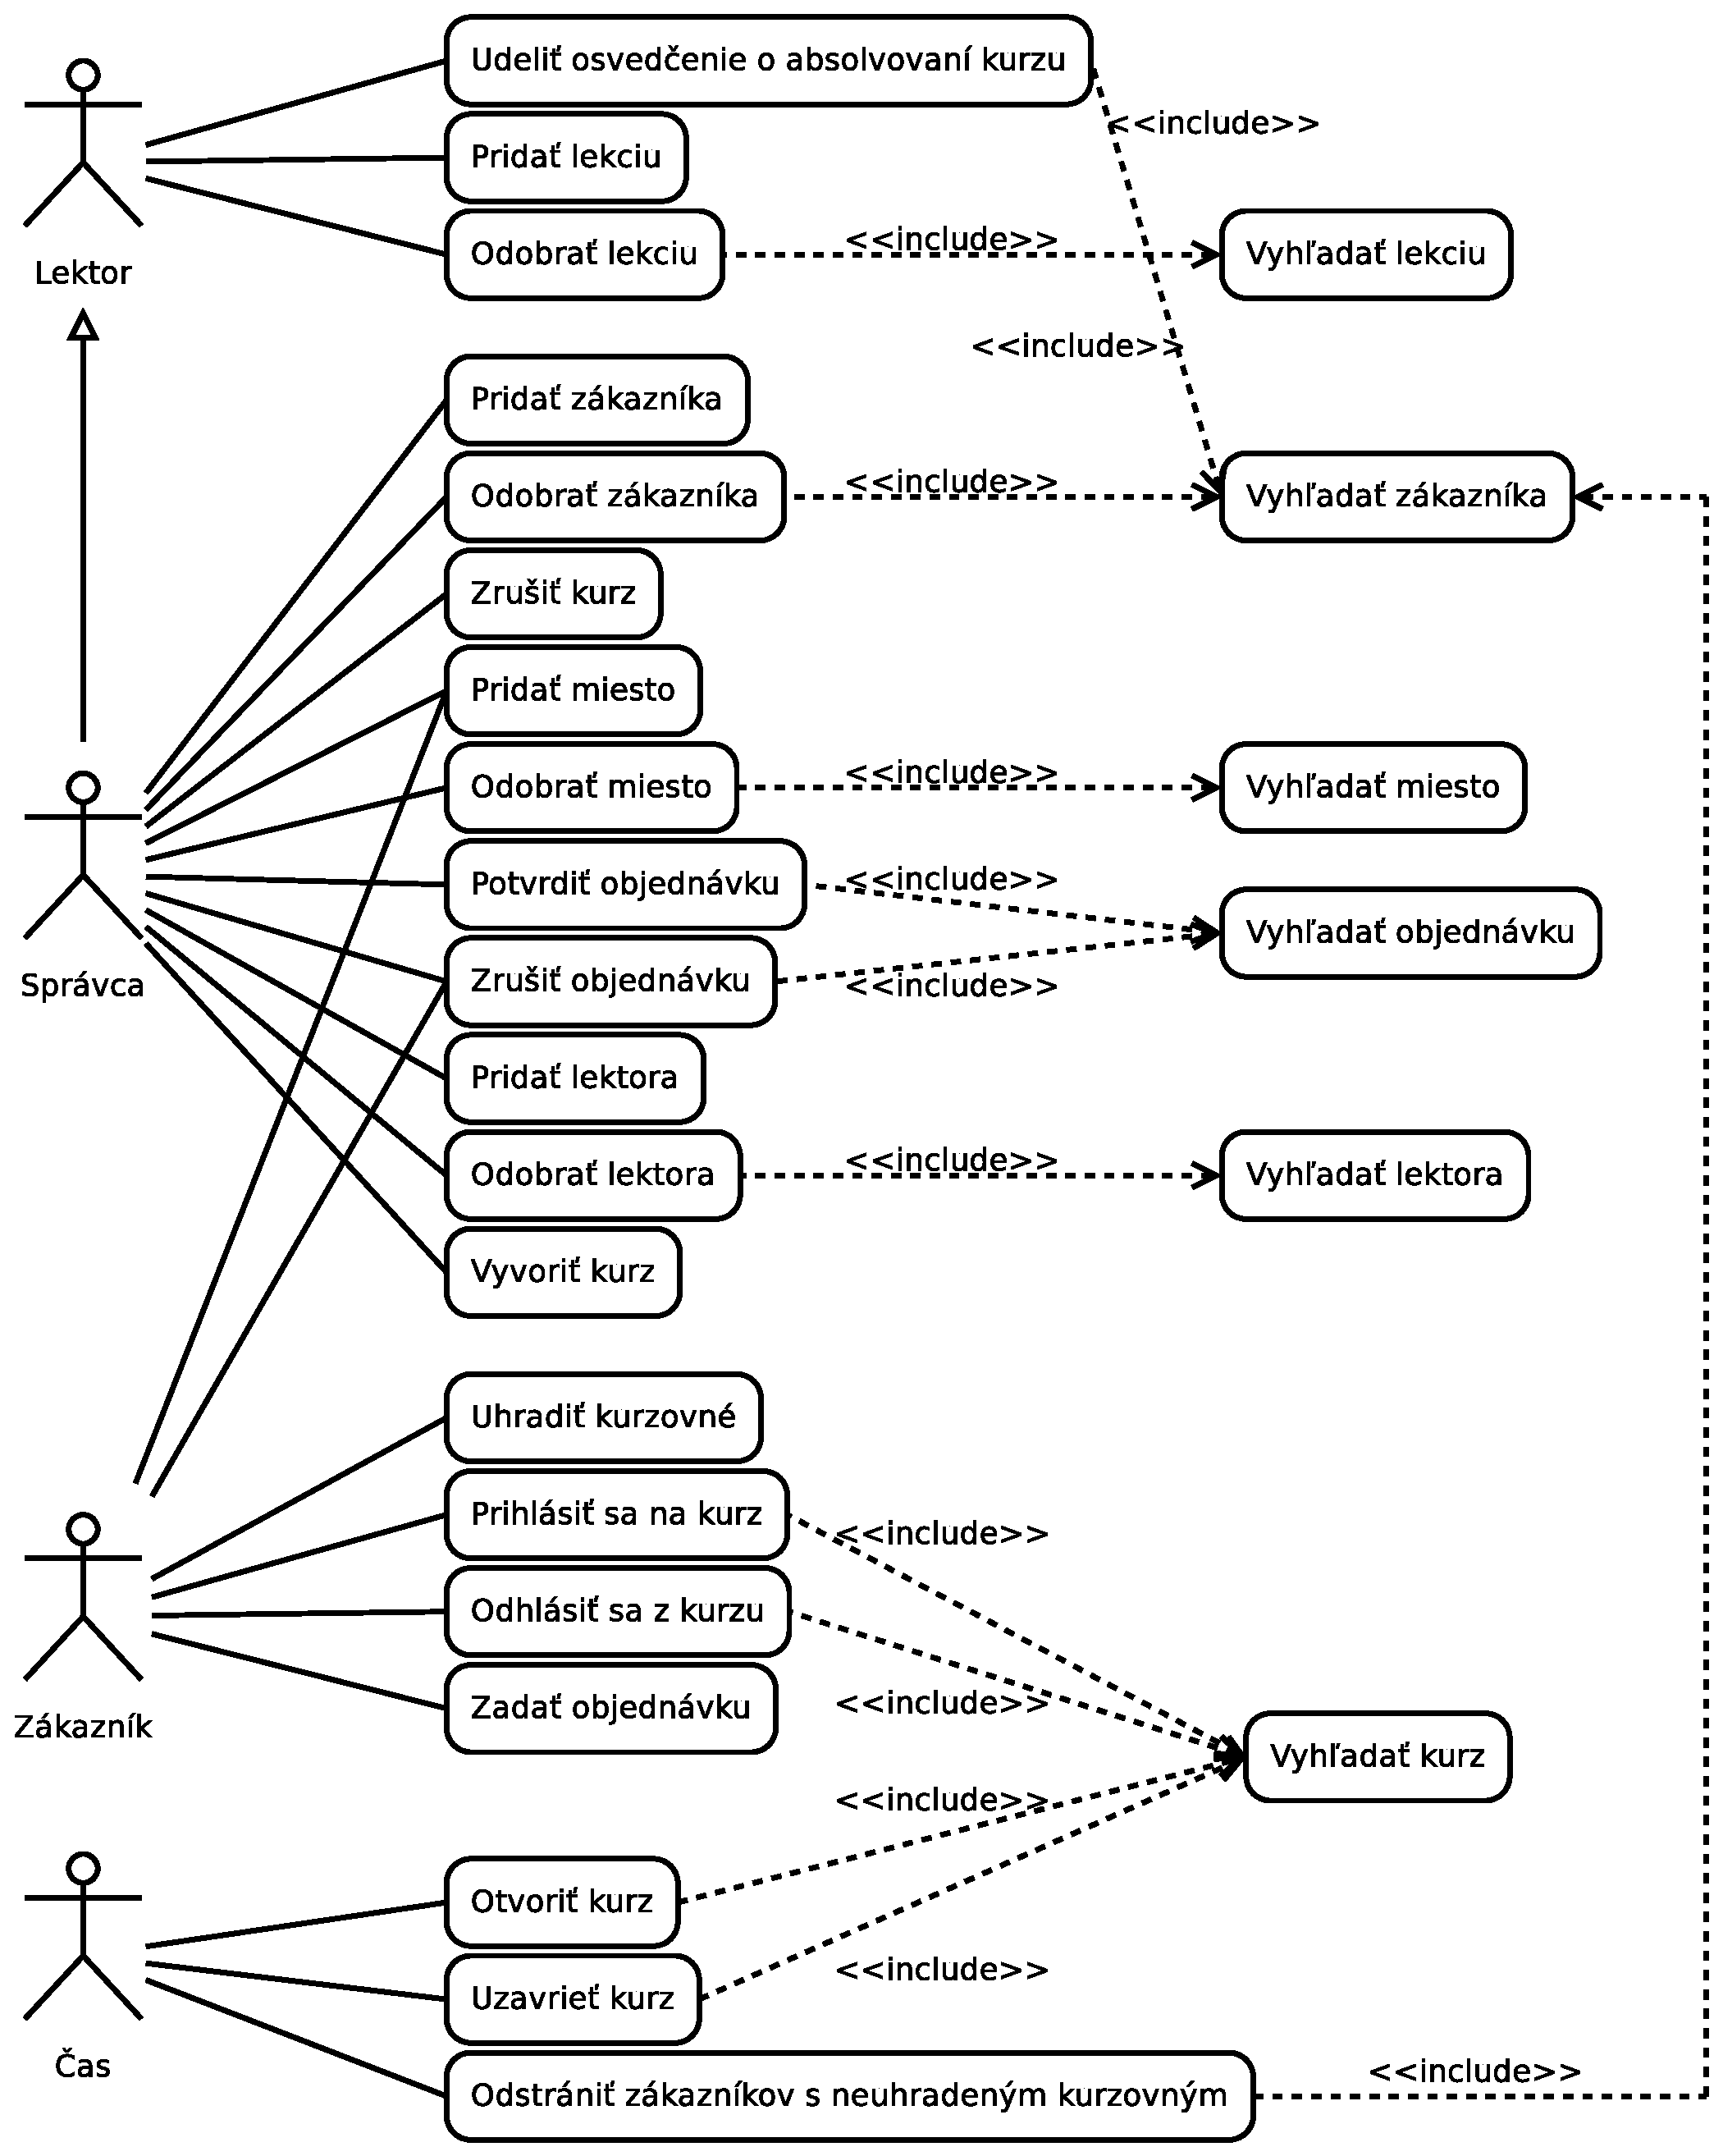
\includegraphics[height=17cm]{img/use_case.eps}
			\captionof{figure}{Diagram prípadov použitia.}
		\end{center}
	\subsubsection{Plán projektu}
Žeby 2 iterácie? :D
	\subsubsection{1. iterácia}
		\begin{center}
			\captionsetup{type=figure}
			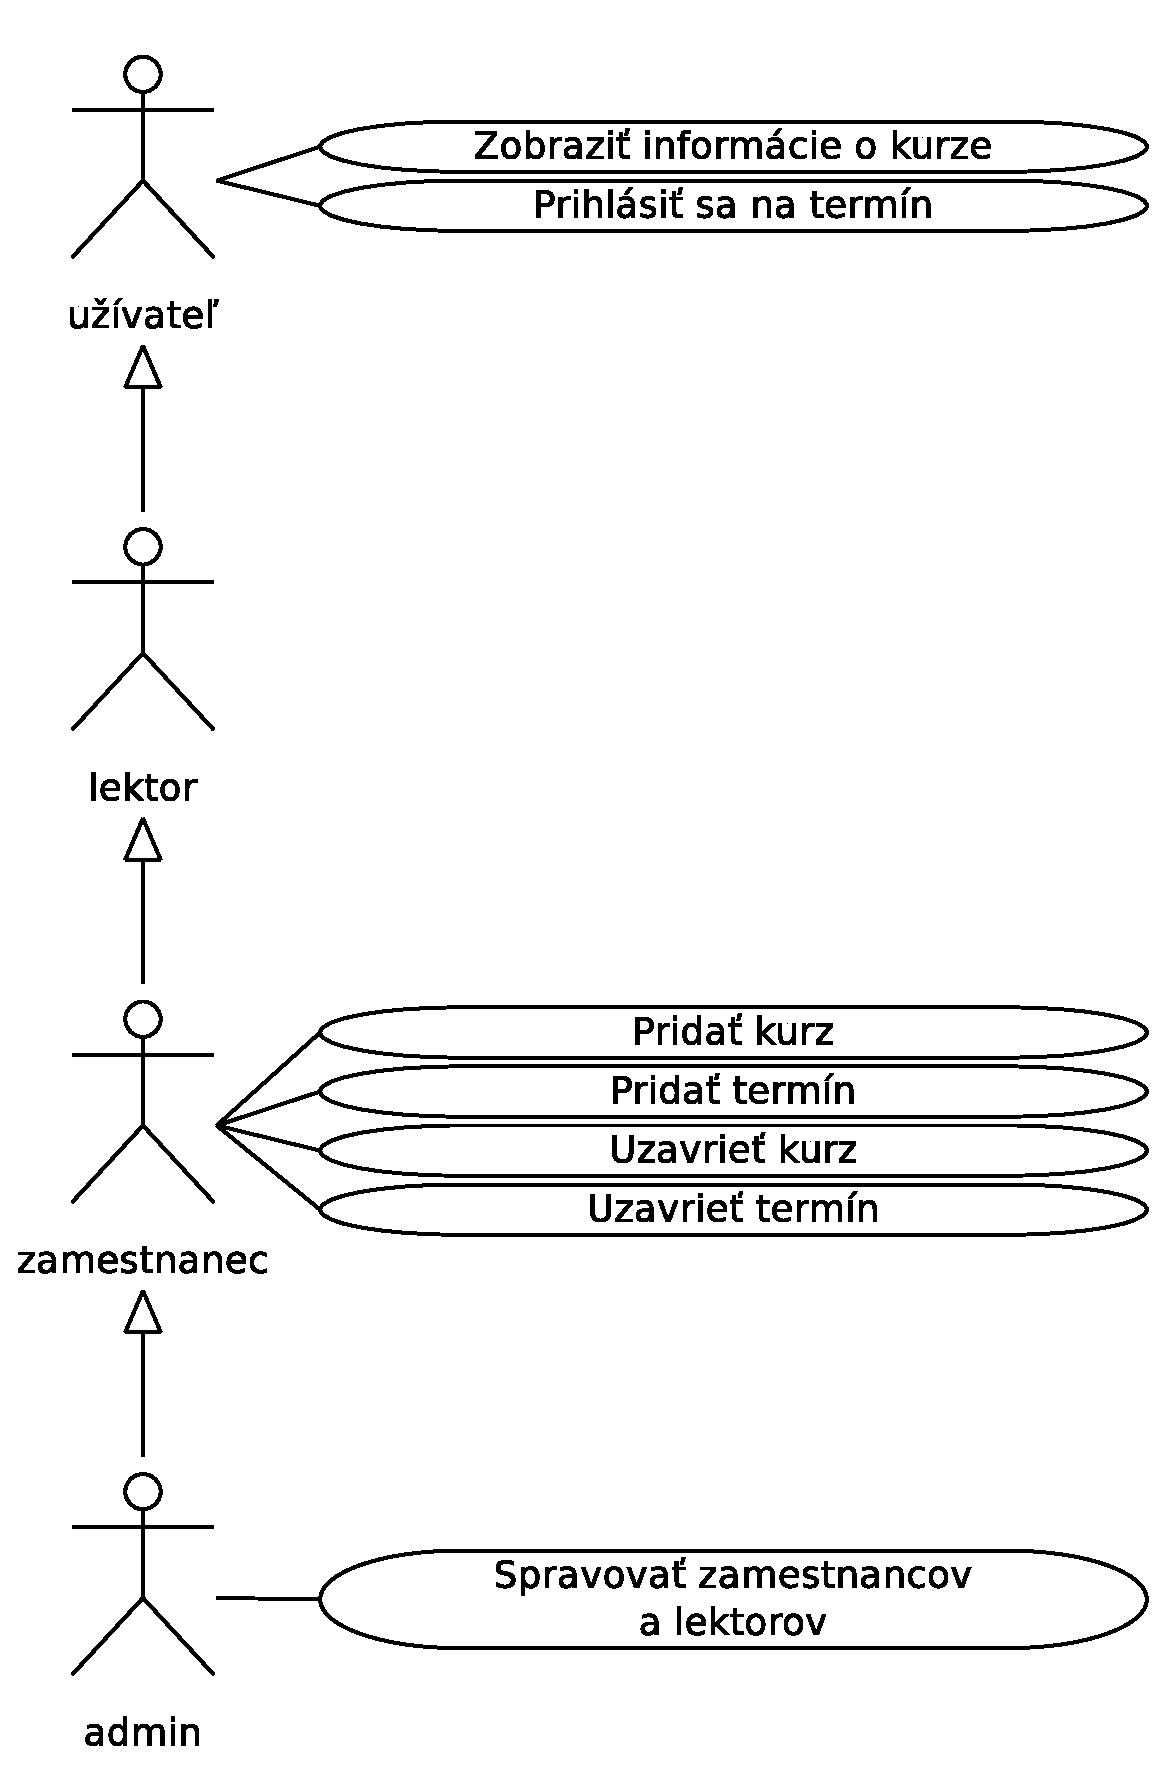
\includegraphics[height=17cm]{img/use_case_iter1.eps}
			\captionof{figure}{Diagram implementovaných prípadov použitia po 1. iterácii.}
		\end{center}
	\subsubsection{2. iterácia}
		\begin{center}
			\captionsetup{type=figure}
			\includegraphics[height=17cm]{img/use_case_iter2.eps}
			\captionof{figure}{Diagram implementovaných prípadov použitia po 2. iterácii.}
		\end{center}
	\subsubsection{3. iterácia}
		\begin{center}
			\captionsetup{type=figure}
			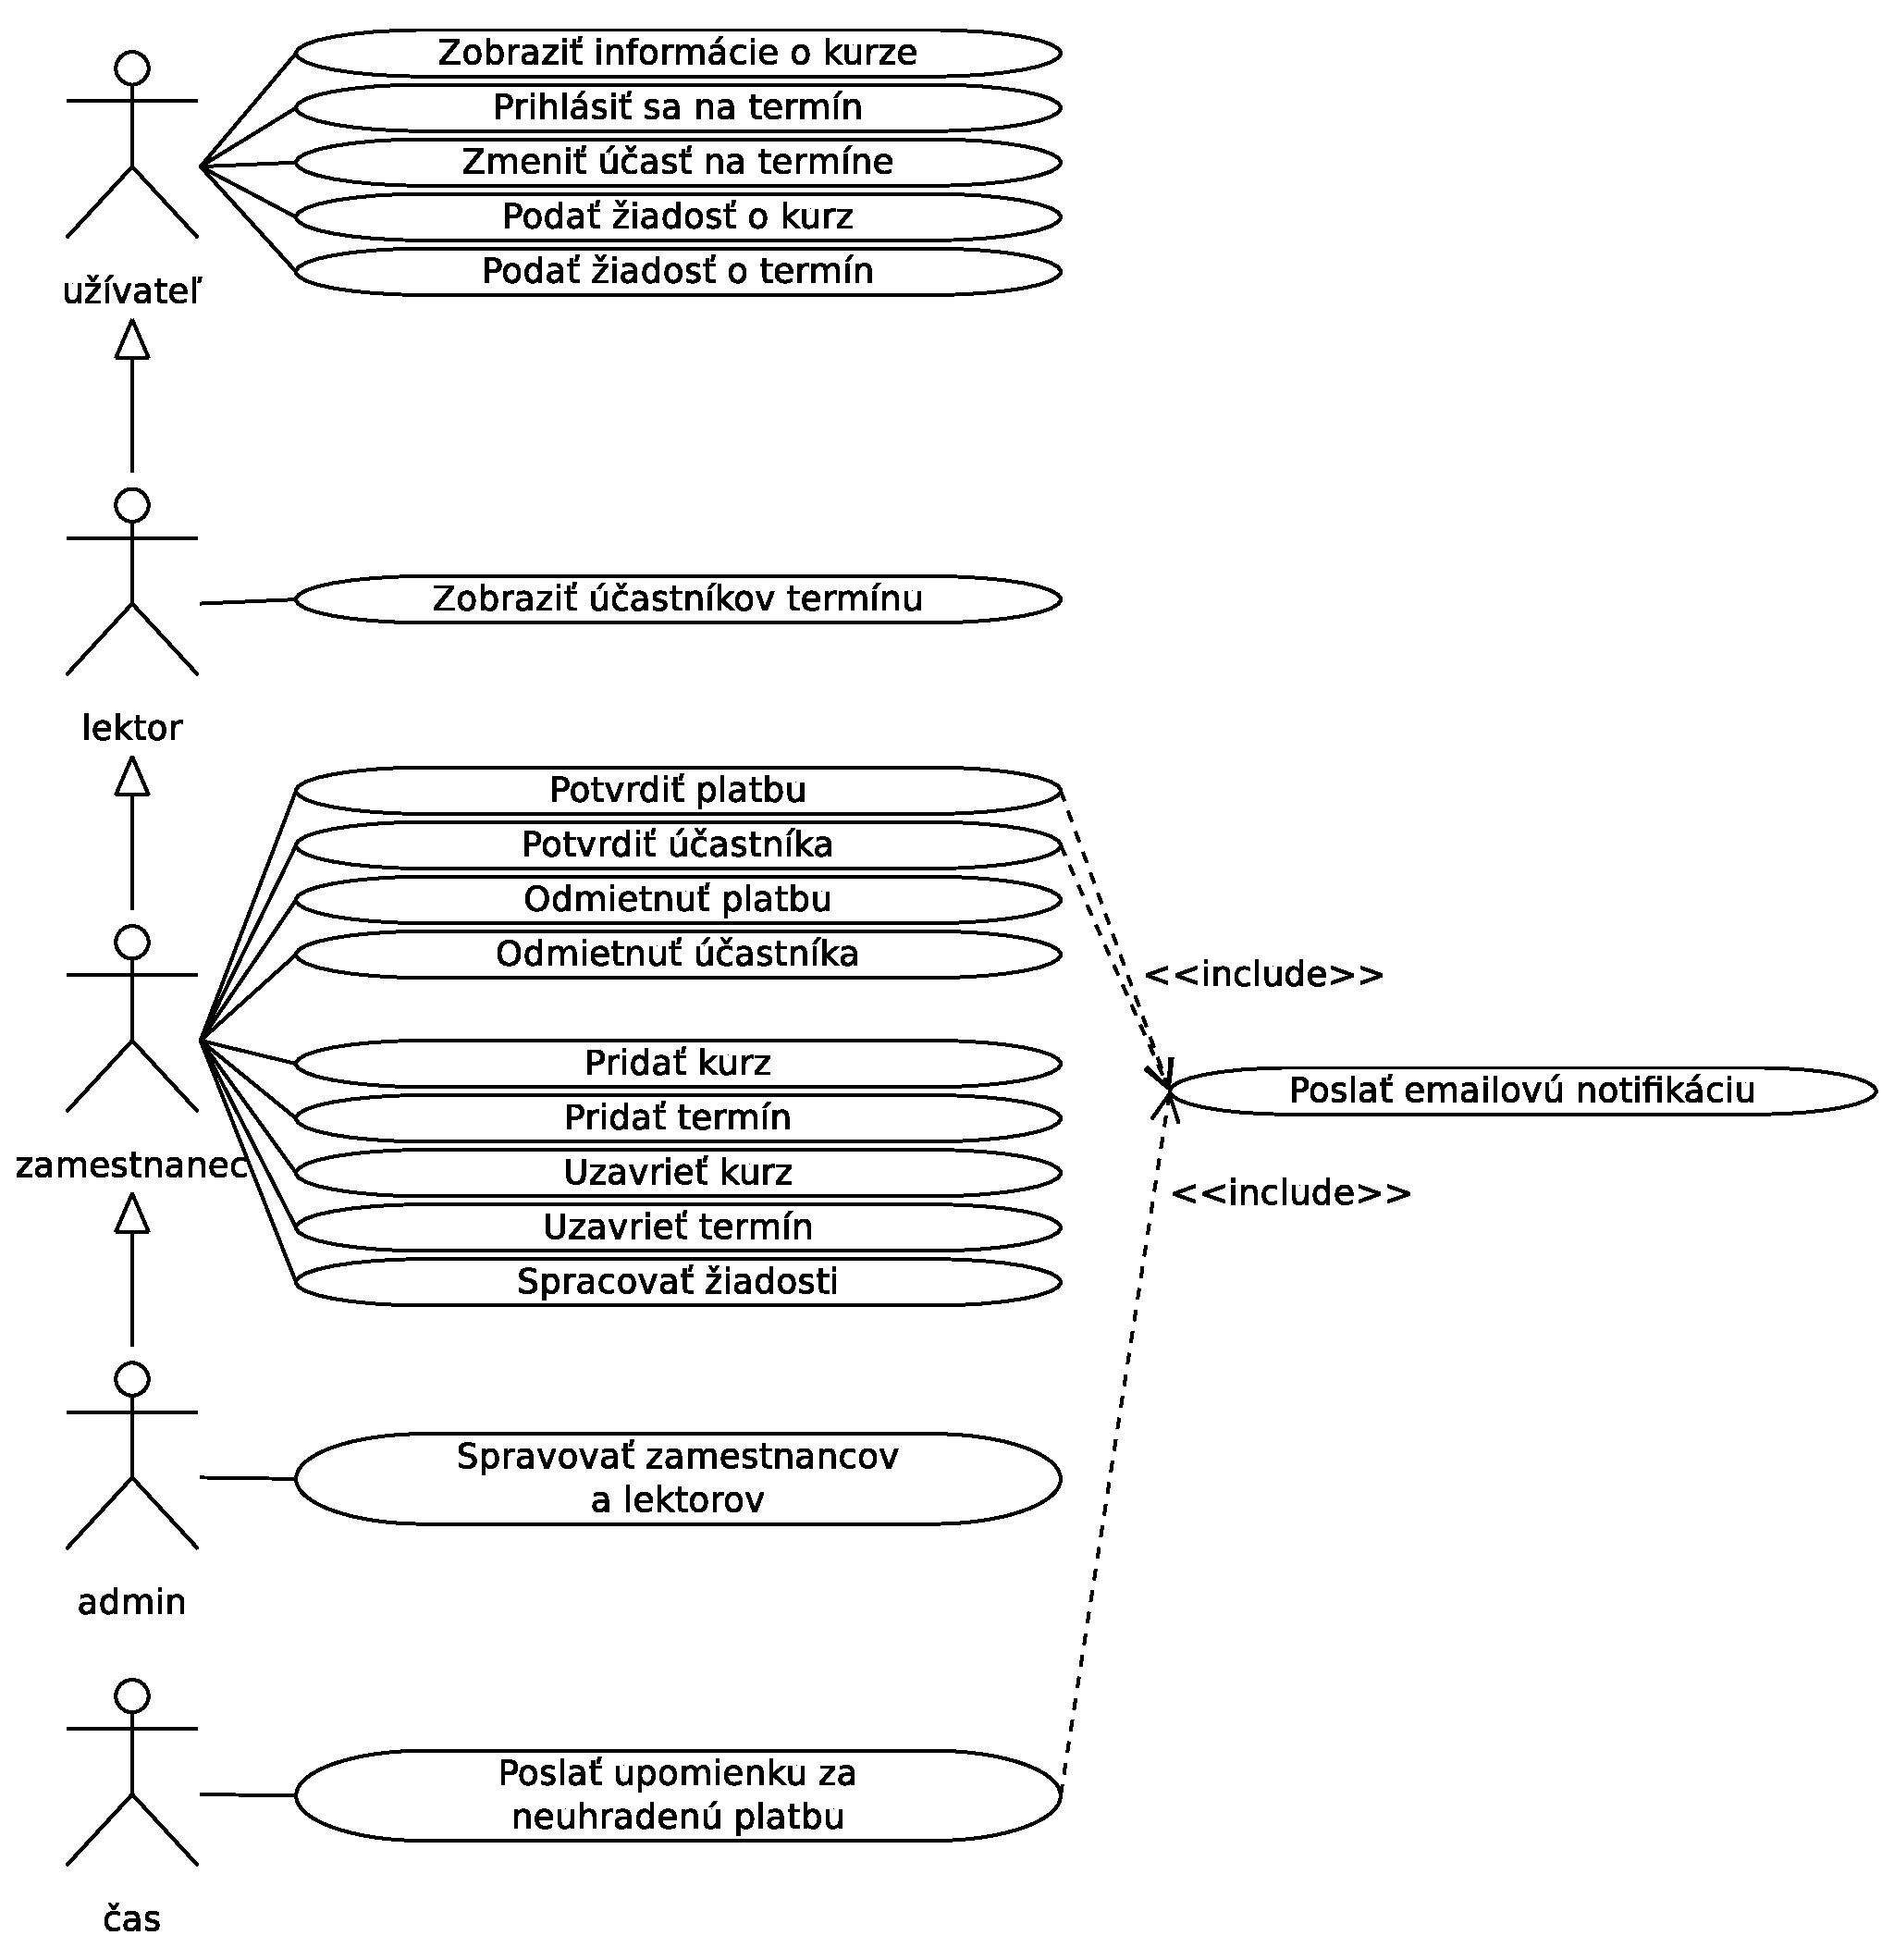
\includegraphics[height=17cm]{img/use_case_iter3.eps}
			\captionof{figure}{Diagram implementovaných prípadov použitia po 3. iterácii.}
		\end{center}
	\subsubsection{4. iterácia}
		\begin{center}
			\captionsetup{type=figure}
			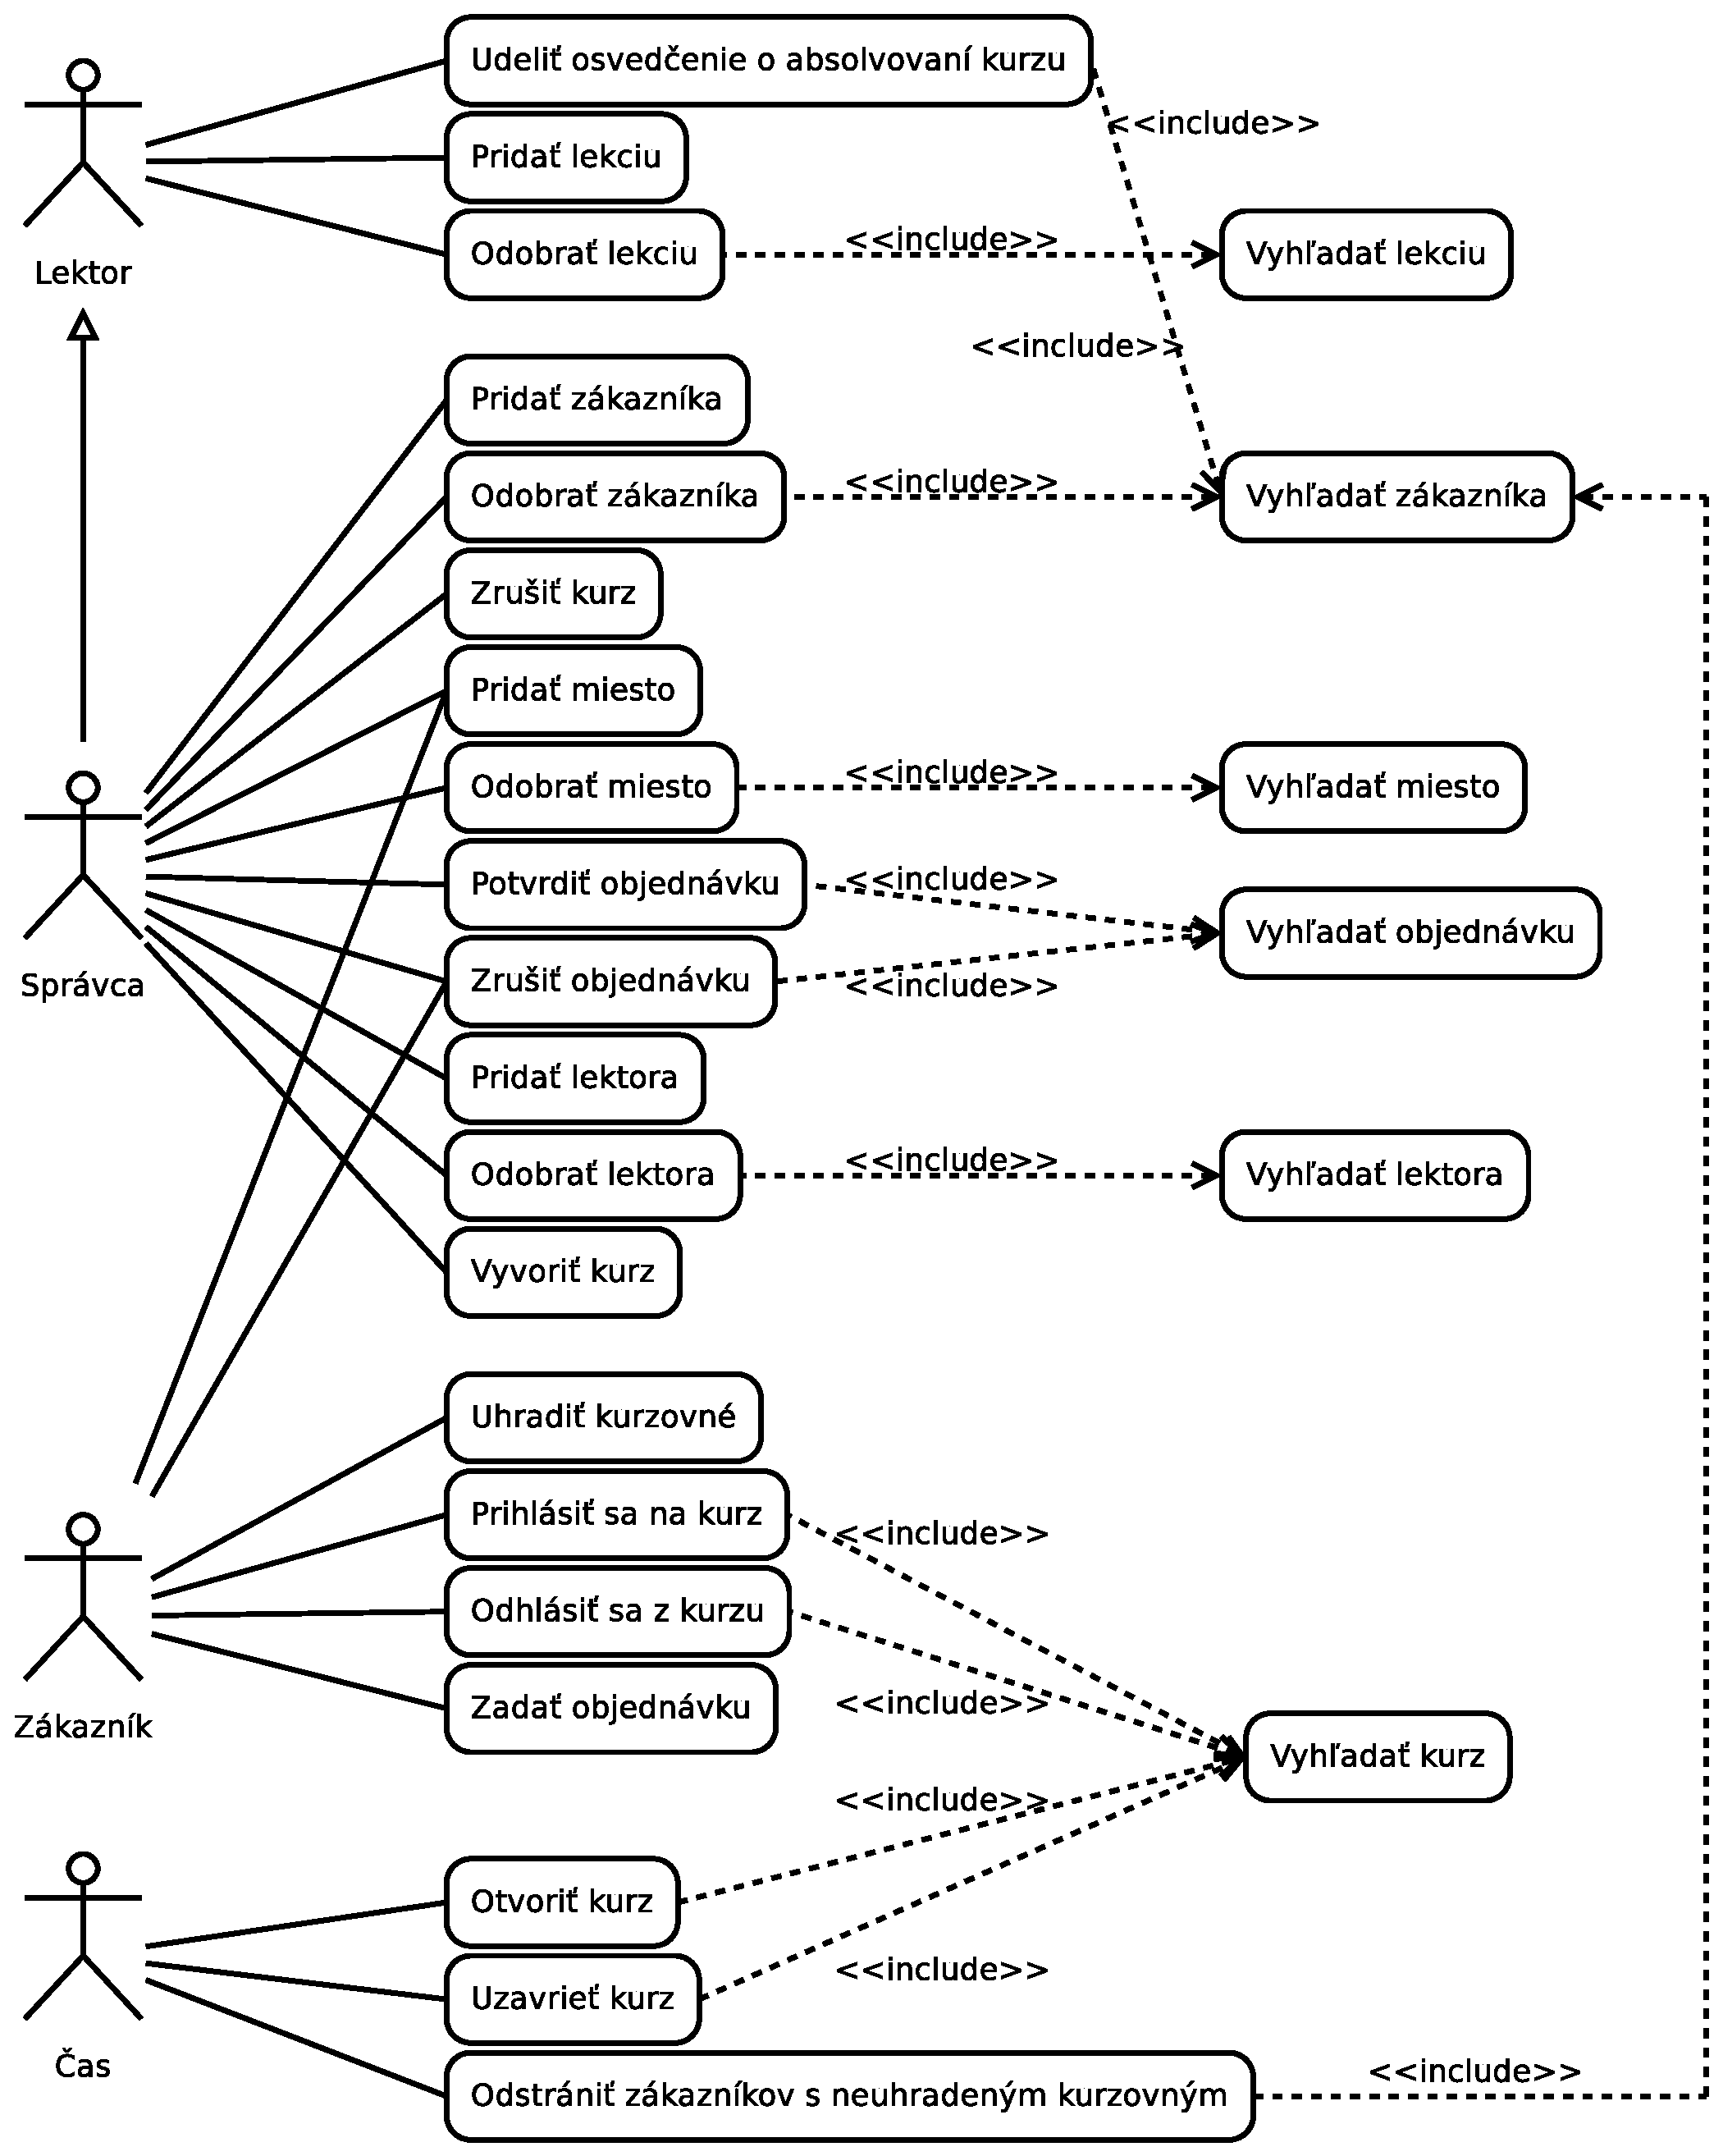
\includegraphics[height=17cm]{img/use_case.eps}
			\captionof{figure}{Diagram implementovaných prípadov použitia po 4. iterácii.}
		\end{center}
\end{document}
